\chapter{Dekomposisi Nilai Singular}
\label{chap:SingularValueDecomposition}

Kita akan menggambarkan cara kerja beberapa transformasi linear
$\map{t}{\Re^2}{\Re^2}$ (kita menggunakan $\Re^2$ karena gambarnya mudah
dibuat).
Kemudian, kita akan memperluas gagasan ini ke dimensi yang lebih tinggi dan
memberikan salah satu akibat praktisnya.


\section{Menggambarkan aksi}
Salah satu sifat yang mendefinisikan peta linear adalah
$h(r\cdot\vec{v})=r\cdot h(\vec{v})$.
Ingat bahwa garis yang melalui titik asal di $\Re^n$ berbentuk
$\set{r\cdot \vec{v}\suchthat r\in\Re}$ untuk suatu~$\vec{v}\neq\zero$.
Jadi, sifat perkalian skalar memberlakukan suatu syarat keseragaman pada peta
linear:~aksinya pada setiap garis yang melalui titik asal ditentukan oleh
aksinya pada salah satu vektor taknol di garis itu.

Sebagai contoh, perhatikan garis~$y=2x$ pada bidang
\begin{equation*}
  \set{r\cdot\colvec{1 \\ 2}\suchthat r\in\Re}
\end{equation*}
dan transformasi $\map{t}{\Re^2}{\Re^2}$ yang direpresentasikan oleh matriks
berikut.
\begin{equation*}
  \rep{t}{\stdbasis_2,\stdbasis_2}
  =
  \begin{mat}
    1 &2 \\
    3 &4
  \end{mat}
\end{equation*}
Jika Anda memilih sebuah vektor domain~$\vec{v}$, menghitung pengaruh~$t$
menjadi mudah.
\begin{equation*}
  \vec{v}=\colvec{1 \\ 2}\mapsunder{t}\colvec{5 \\ 11}
\end{equation*}
Paragraf sebelumnya menyatakan bahwa pada $2\vec{v}$, peta tersebut memberi
pengaruh dua kali lipat; pada $3\vec{v}$, pengaruhnya tiga kali lipat; dan
seterusnya.
\begin{equation*}
  \colvec{2 \\ 4}\mapsunder{t}\colvec{10 \\ 22}
  \qquad
  \colvec{3 \\ 6}\mapsunder{t}\colvec{15 \\ 33}
  \qquad
  \colvec{r \\ 2r}\mapsunder{t}\colvec{5r \\ 11r}
\end{equation*}

%% The $t(r\cdot\vec{v})=r\cdot t(\vec{v})$ relationship says that
%% a linear map has the same effect on all vectors in a line through the
%% origin.
Jadi, untuk menggambarkan aksi suatu peta pada seluruh bidang, kita akan
memilih satu vektor taknol~$\vec{v}$ dari setiap garis yang melalui titik asal
dan menunjukkan ke mana transformasi membawanya.
Himpunan alami yang memuat satu titik dari setiap garis yang melalui titik
asal adalah setengah lingkaran satuan bagian atas, seperti ditunjukkan di sini
(warna-warnanya dijelaskan di bawah).
\begin{sagesilent}
load("plot_action.sage")
p = plot_circle_action(1,0,0,1) 
p.set_axes_range(-1.5, 1.5, -0.5, 1.5) 
p.save("graphics/svd000.pdf")
\end{sagesilent}
\begin{equation*}
  U=\set{\vec{v}=\colvec{\cos(t) \\ \sin(t)}
         \suchthat 
         0\leq t<\pi}
  \qquad
  \vcenteredhbox{\includegraphics{graphics/svd000.pdf}}  
\end{equation*}
Untuk memperoleh tepat satu wakil bagi sumbu~$x$, titik $(1,0)$ dimasukkan ke
dalam himpunan tersebut, sedangkan $(-1,0)$ tidak.

Transformasi pertama yang akan kita ilustrasikan sederhana.
\begin{equation*}
  \colvec{x \\ y} \mapsunder{t} \colvec{2x \\ y}
\end{equation*}
Kode di bawah memuat \inlinecode{plot_action.sage} agar fungsi
\inlinecode{plot_circle_action(a,b,c,d)} dapat digunakan.
Fungsi ini membagi setengah lingkaran masukan bagian atas menjadi beberapa
bagian---bagian merah, jingga, dan seterusnya---lalu mengalikan titik-titik
pada ruas-ruas lengkung itu dengan matriks berikut
\begin{equation*}
  \begin{mat}
    a &b \\
    c &d
  \end{mat}
\end{equation*}
(untuk transformasi pertama ini kita ambil $a=2$, $b=0$, $c=0$, dan $d=1$).
Terakhir, fungsi tersebut menyambungkan ruas-ruas keluaran untuk memperoleh
kurva keluaran; ruas-ruas keluarannya diberi warna merah, jingga, dan
seterusnya.
Daftar kode sumber lengkap \inlinecode{plot_action.sage} terdapat di akhir
bab ini.

Untuk menampilkan gambar sebelum dan sesudah, kode tersebut mula-mula
memplot lingkaran tanpa perubahan, yakni di bawah pengaruh peta identitas,
lalu memplot hasil penerapan transformasi.
\begin{sagecommandline}
sage: load("plot_action.sage")
sage: q = plot_circle_action(1,0,0,1) 
sage: q.set_axes_range(-2, 2, -1, 2) 
sage: q.save("graphics/svd001a.pdf")
sage: p = plot_circle_action(2,0,0,1) 
sage: p.set_axes_range(-2, 2, -1, 2) 
sage: p.save("graphics/svd001b.pdf")
\end{sagecommandline}
% \begin{sagesilent}
% load("plot_action.sage")
% q = plot_circle_action(1,0,0,1) 
% q.set_axes_range(-2, 2, -1, 2) 
% q.save("graphics/svd001a.pdf")
% p = plot_circle_action(2,0,0,1) 
% p.set_axes_range(-2, 2, -1, 2) 
% p.save("graphics/svd001b.pdf")
% \end{sagesilent}
Berikut gambar sebelum dan sesudahnya.
Warna-warna tersebut memperlihatkan keterkaitannya\Dash yaitu titik mana di
sebelah kiri yang dipetakan ke titik mana di sebelah kanan.
\begin{equation*}
  \vcenteredhbox{\includegraphics{graphics/svd001a.pdf}}
  \quad\mapsunder{\big (\begin{smallmatrix} 2 &0 \\ 0 &1 \end{smallmatrix}\big )}\quad
  \vcenteredhbox{\includegraphics{graphics/svd001b.pdf}}
\end{equation*}
Peta ini meregangkan objek pada arah~$x$ dengan faktor dua.

Selanjutnya kita tampilkan aksi peta
\begin{equation*}
  \colvec{x \\ y} \mapsto \colvec{-x \\ 3y}
\end{equation*}
yang melipatgandakan komponen~$y$ menjadi tiga kali dan juga mengalikan
komponen~$x$ dengan $-1$.\footnote{%
  Seperti pada bab-bab lain, sebagian gambar dibuat dengan beberapa opsi yang
  tidak ditampilkan.
  Dalam kasus ini, kedua perintah \protect\inlinecode{p.save(...)} memiliki
  opsi \protect\inlinecode{ticks\_integer=True}.
  Opsi-opsi ini tidak ditampilkan semata-mata untuk mengurangi rincian yang
  bukan merupakan aljabar linear.}
\begin{sagecommandline}
sage: q = plot_circle_action(1,0,0,1) 
sage: q.set_axes_range(-2, 2, -1.25, 3.25) 
sage: q.save("graphics/svd002a.pdf")
sage: p = plot_circle_action(-1,0,0,3) 
sage: p.set_axes_range(-2, 2, -1.25, 3.25) 
sage: p.save("graphics/svd002b.pdf")
\end{sagecommandline}
\begin{sagesilent}
load("plot_action.sage")
q = plot_circle_action(1,0,0,1) 
q.set_axes_range(-2, 2, -1.25, 3.25) 
q.save("graphics/svd002a.pdf", ticks_integer=True)
p = plot_circle_action(-1,0,0,3) 
p.set_axes_range(-2, 2, -1.25, 3.25) 
p.save("graphics/svd002b.pdf", ticks_integer=True)
\end{sagesilent}
\begin{equation*}
  \vcenteredhbox{\includegraphics{graphics/svd002a.pdf}}
  \quad\mapsunder{\big (\begin{smallmatrix} -1 &0 \\ 0 &3 \end{smallmatrix}\big )}\quad
  \vcenteredhbox{\includegraphics{graphics/svd002b.pdf}}
\end{equation*}
Melipatgandakan komponen~$y$ menjadi tiga kali mudah dipahami.
Untuk pengambilan negatif komponen~$x$, warna-warna menjadi sangat berguna.
Pada lingkaran masukan, ketika Anda bergerak berlawanan arah jarum jam,
warnanya berurutan dari merah ke jingga, hijau, biru, nila, lalu ungu.
Namun, pada keluaran urutannya berlawanan:~ketika bergerak berlawanan arah
jarum jam, warnanya beralih dari ungu ke merah.
Transformasi ini mengubah orientasi, atau ``arah'', kurva.

Transformasi berikutnya adalah rotasi sebesar $\pi/4$~radian searah jarum jam.
\begin{equation*}
  \colvec{x \\ y} \mapsto \colvec{\cos(-\pi/4)\cdot x-\sin(-\pi/4)\cdot y \\
                                                   \sin(-\pi/4)\cdot x+\cos(-\pi/4)\cdot y}
\end{equation*}
\begin{sagecommandline}
sage: q = plot_circle_action(1,0,0,1) 
sage: q.set_axes_range(-1.5, 1.5, -1, 1.5) 
sage: q.save("graphics/svd003a.pdf")
sage: p = plot_circle_action(cos(-pi/4),-sin(-pi/4),sin(-pi/4),cos(-pi/4)) 
sage: p.set_axes_range(-1.5, 1.5, -1, 1.5) 
sage: p.save("graphics/svd003b.pdf")
\end{sagecommandline}
\begin{equation*}
  \vcenteredhbox{\includegraphics{graphics/svd003a.pdf}}
  \quad\mapsunder{\big (\begin{smallmatrix} \cos(-\pi/4) &-\sin(-\pi/4) \\ \sin(-\pi/4) &\cos(-\pi/4) \end{smallmatrix}\big )}\quad
  \vcenteredhbox{\includegraphics{graphics/svd003b.pdf}}
\end{equation*}

Transformasi berikutnya adalah sebuah geseran.\footnote{%
  Geseran adalah gerak dua bagian suatu benda ketika keduanya bergeser relatif
  satu sama lain dalam arah yang sejajar dengan bidang kontaknya.
  Susunlah setumpuk koran dan dorong tumpukan itu dari samping.
  Lembar-lembar kertas akan bergeser sejajar satu sama lain, dan lembar paling
  atas bergeser paling jauh.}
\begin{equation*}
  \colvec{x \\ y} \mapsto \colvec{x+2y \\ y}
\end{equation*}
Karena komponen keluaran pertama memuat $2y$, komponen pertama vektor masukan
dengan nilai mutlak~$y$ yang besar terpengaruh lebih kuat daripada komponen
pertama vektor masukan yang dekat dengan sumbu~$x$.
\begin{sagecommandline}
sage: q = plot_circle_action(1,0,0,1) 
sage: q.set_axes_range(-1.5, 2.5, -.25, 1.25) 
sage: q.save("graphics/svd004a.pdf")
sage: p = plot_circle_action(1,2,0,1) 
sage: p.set_axes_range(-1.5, 2.5, -.25, 1.25) 
sage: p.save("graphics/svd004b.pdf")
\end{sagecommandline}
\begin{sagesilent}
load("plot_action.sage")
q = plot_circle_action(1,0,0,1) 
q.set_axes_range(-1.5, 2.5, -.25, 2.25) 
q.save("graphics/svd004a.pdf", ticks_integer=True)
p = plot_circle_action(1,2,0,1) 
p.set_axes_range(-1.5, 2.5, -.25, 2.25) 
p.save("graphics/svd004b.pdf", ticks_integer=True)
\end{sagesilent}
\begin{equation*}
  \vcenteredhbox{\includegraphics{graphics/svd004a.pdf}}
  \quad\mapsunder{\big (\begin{smallmatrix} 1 &2 \\ 0 &1 \end{smallmatrix}\big )}\quad
  \vcenteredhbox{\includegraphics{graphics/svd004b.pdf}}
\end{equation*}

Berikutnya adalah geseran yang memengaruhi komponen kedua keluaran, kali ini
menurut jarak masukan dari sumbu~$x$.
\begin{equation*}
  \colvec{x \\ y} \mapsto \colvec{x \\ (1/2)x+y}
\end{equation*}
\begin{sagecommandline}
sage: q = plot_circle_action(1,0,0,1) 
sage: q.set_axes_range(-1.25, 1.25, -0.75, 1.5) 
sage: q.save("graphics/svd005a.pdf")
sage: p = plot_circle_action(1,0,1/2,1) 
sage: p.set_axes_range(-1.25, 1.25, -0.75, 1.5) 
sage: p.save("graphics/svd005b.pdf")
\end{sagecommandline}
% \begin{sagesilent}
% load("plot_action.sage")
% q = plot_circle_action(1,0,0,1) 
% q.set_axes_range(-2, 2, -2, 2) 
% q.save("graphics/svd005a.pdf")
% p = plot_circle_action(1,0,1/2,1) 
% p.set_axes_range(-2, 2, -2, 2) 
% p.save("graphics/svd005b.pdf")
% \end{sagesilent}
\begin{equation*}
  \vcenteredhbox{\includegraphics{graphics/svd005a.pdf}}
  \quad\mapsunder{\big (\begin{smallmatrix} 1 &0 \\ 1/2 &1 \end{smallmatrix}\big )}\quad
  \vcenteredhbox{\includegraphics{graphics/svd005b.pdf}}
\end{equation*}

Dan berikut sebuah peta umum.
\begin{sagecommandline}
sage: q = plot_circle_action(1,0,0,1) 
sage: q.set_axes_range(-2, 4, -3, 6) 
sage: q.save("graphics/svd006a.pdf")
sage: p = plot_circle_action(1,2,3,4) 
sage: p.set_axes_range(-2, 4, -3, 6) 
sage: p.save("graphics/svd006b.pdf")
\end{sagecommandline}
% \begin{sagesilent}
% load("plot_action.sage")
% q = plot_circle_action(1,0,0,1) 
% q.set_axes_range(-2, 4, -3, 6) 
% q.save("graphics/svd006a.pdf",figsize=3)
% p = plot_circle_action(1,2,3,4) 
% p.set_axes_range(-2, 4, -3, 6) 
% p.save("graphics/svd006b.pdf",figsize=3)
% \end{sagesilent}
\begin{equation*}
  \vcenteredhbox{\includegraphics{graphics/svd006a.pdf}}
  \quad\mapsunder{\big (\begin{smallmatrix} 1 &2 \\ 3 &4 \end{smallmatrix}\big )}\quad
  \vcenteredhbox{\includegraphics{graphics/svd006b.pdf}}
\end{equation*}
Selain merotasi dan menggeser, peta ini juga mengubah orientasi.



\section{SVD}
Pada gambar-gambar tersebut, bayangan setengah lingkaran adalah setengah
elips; akibatnya, bayangan lingkaran penuh adalah sebuah elips.
Ingat bahwa di $\Re^2$, sebuah elips memiliki sumbu mayor, yakni sumbu yang
lebih panjang, dan sumbu minor.\footnote{%
  Jika kedua sumbu sama panjang, elips tersebut adalah lingkaran.
  Jika salah satu sumbu panjangnya nol, elips tersebut adalah ruas garis;
  jika keduanya panjangnya nol, elips tersebut adalah sebuah titik.}
Nyatakan panjang semisumbu mayor dengan $\sigma_1$, yaitu jarak dari pusat
ke titik terjauh pada elips, dan nyatakan panjang semisumbu minor dengan
$\sigma_2$.
\begin{sagecommandline}
sage: plot.options['axes_pad'] = 0.5
sage: plot.options['fontsize'] = 4
sage: plot.options['aspect_ratio'] = 1
sage: sigma_1=3
sage: sigma_2=1
sage: E = ellipse((0,0), sigma_1, sigma_2)
sage: E.save("graphics/svd100.pdf")
\end{sagecommandline}
\begin{sagesilent}
plot.options['axes_pad'] = 0.5
plot.options['fontsize'] = 2
plot.options['aspect_ratio'] = 1
plot.options['figsize'] = 1
sigma_1=3
sigma_2=1
E = ellipse((0,0), sigma_1, sigma_2)
# E.save("graphics/svd100.pdf", axes_pad=0.075, dpi=1200, fontsize=7, ticks=([-3,-2,-1,1,2,3],[-1,1]), figsize=1.5)
E.save("graphics/svd100.pdf", ticks_integer=True, axes_pad=0.075, figsize=3)
\end{sagesilent}
\begin{center}
  \includegraphics{graphics/svd100.pdf}
\end{center}
Kedua sumbu itu ortogonal.
Pada gambar di atas, sumbu mayor terletak pada sumbu~$x$, sedangkan sumbu
minor terletak pada sumbu~$y$.

Di bawah setiap peta linear $\map{t}{\Re^n}{\Re^m}$, bola satuan dipetakan
ke sebuah hiperelips.
Hal ini merupakan salah satu bentuk \textit{Dekomposisi Nilai Singular}
matriks:~untuk setiap peta linear $\map{t}{\Re^n}{\Re^m}$, terdapat basis
$B=\sequence{\vec{\beta}_1,\ldots,\vec{\beta}_n}$ bagi domain dan
$D=\sequence{\vec{\delta}_1,\ldots,\vec{\delta}_m}$ bagi kodomain sehingga
$t(\vec{\beta}_i)=\sigma_i\vec{\delta}_i$ untuk
$i\leq\min(m,n)$; jika $n>m$, vektor basis domain yang tersisa dipetakan ke
nol. Skalar $\sigma_i$ disebut \textit{nilai singular}.
Bagian berikutnya memberikan garis besar pembuktiannya, tetapi mula-mula
kita ilustrasikan hasil ini dengan sebuah matriks contoh.
\Sage{} akan menemukan kedua basis $B$ dan~$D$ serta menggambarkan bagaimana
vektor $\vec{\beta}_i$ dipetakan ke $\sigma_i\vec{\delta}_i$.

Jadi, perhatikan kembali matriks umum tadi.
Berikut aksinya sekali lagi, kini ditampilkan pada lingkaran penuh.
\begin{sagecommandline}
sage: load("plot_action.sage")
sage: q = plot_circle_action(1,0,0,1,full_circle=True) 
sage: q.set_axes_range(-3, 3, -5, 5) 
sage: q.save("graphics/svd101a.pdf")
sage: p = plot_circle_action(1,2,3,4,full_circle=True) 
sage: p.set_axes_range(-3, 3, -5, 5) 
sage: p.save("graphics/svd101b.pdf")
\end{sagecommandline}
\begin{sagesilent}
load("plot_action.sage")
q = plot_circle_action(1,0,0,1,full_circle=True) 
q.set_axes_range(-3, 3, -5, 5) 
q.save("graphics/svd101a.pdf", ticks_integer=True)
p = plot_circle_action(1,2,3,4,full_circle=True) 
p.set_axes_range(-3, 3, -5, 5) 
p.save("graphics/svd101b.pdf", ticks_integer=True)
\end{sagesilent}
\begin{equation*}
  \vcenteredhbox{\includegraphics{graphics/svd101a.pdf}}
  \quad\mapsunder{\big (\begin{smallmatrix} 1 &2 \\ 3 &4 \end{smallmatrix}\big )}\quad
  \vcenteredhbox{\includegraphics{graphics/svd101b.pdf}}
  \tag{$*$}
\end{equation*}
\Sage{} akan mencari SVD matriks contoh ini.
\begin{sagecommandline}
sage: M = matrix(RDF, [[1, 2], [3, 4]])
sage: U,Sigma,V = M.SVD()
sage: U
sage: Sigma
sage: V
sage: U*Sigma*(V.transpose())
\end{sagecommandline}
\noindent 
Dekomposisi Nilai Singular menyatakan $M$ sebagai hasil kali tiga matriks,
$U\Sigma\trans{V}$.
Vektor basis domain $\vec{\beta}_1$ dan $\vec{\beta}_2$ adalah kolom-kolom
$V$, sedangkan vektor basis kodomain $\vec{\delta}_1$ dan
$\vec{\delta}_2$ adalah kolom-kolom $U$.
Nilai singular adalah entri-entri diagonal~$\Sigma$.

Kita dapat meminta \Sage{} memplot pengaruh transformasi terhadap
vektor-vektor basis domain agar dapat dibandingkan dengan vektor-vektor
basis kodomain.
\begin{sagecommandline}
sage: M = matrix(RDF, [[1, 2], [3, 4]])
sage: U,Sigma,V = M.SVD()
sage: beta_1 = vector(RDF, [V[0][0], V[1][0]])
sage: beta_2 = vector(RDF, [V[0][1], V[1][1]])
sage: delta_1 = vector(RDF, [U[0][0], U[1][0]])
sage: delta_2 = vector(RDF, [U[0][1], U[1][1]])
sage: C = circle((0,0), 1)
sage: P = C + plot(beta_1) + plot(beta_2)
sage: P.save("graphics/svd102a.pdf")
sage: image_color=Color(1,0.5,0.5)   # warna untuk t(beta_1), t(beta_2)
sage: Q = C + plot(M*beta_1, width=3) 
sage: Q = Q + plot(delta_1,width=1.4) 
sage: Q = Q + plot(M*beta_2,width=3) 
sage: Q = Q + plot(delta_2,width=1.4)
sage: Q.save("graphics/svd102b.pdf")
\end{sagecommandline}
\begin{sagesilent}
M = matrix(RDF, [[1, 2], [3, 4]])
U,Sigma,V = M.SVD()
beta_1 = vector(RDF, [V[0][0], V[1][0]])
beta_2 = vector(RDF, [V[0][1], V[1][1]])
delta_1 = vector(RDF, [U[0][0], U[1][0]])
delta_2 = vector(RDF, [U[0][1], U[1][1]])
plot.options['axes_pad'] = 0.05
plot.options['fontsize'] = 7
plot.options['aspect_ratio'] = 1
s = 2  # uniform arrowsize
C = circle((0,0), 1)
P = C + plot(beta_1,arrowsize=s) + plot(beta_2,arrowsize=s)
P.save("graphics/svd102a.pdf",figsize=2, ticks_integer=True)
image_color=Color(1,0.5,0.5)   # warna untuk t(beta_1), t(beta_2)
Q = C + plot(M*beta_1, width=3,color=image_color,arrowsize=s) 
Q = Q + plot(delta_1,width=1.4,color='blue',arrowsize=s) 
Q = Q + plot(M*beta_2,width=3,color=image_color,arrowsize=s) 
Q = Q + plot(delta_2,width=1.4,color='blue',arrowsize=s)
Q.save("graphics/svd102b.pdf",figsize=4.467, ticks_integer=True)
\end{sagesilent}
Di bawah, basis domain di sebelah kiri adalah vektor-vektor
$\vec{\beta}$ berwarna biru.
Di sebelah kanan, basis kodomain adalah vektor-vektor $\vec{\delta}$ berwarna
biru. Masih di sebelah kanan, bayangan vektor-vektor $\vec{\beta}$
ditampilkan dengan warna merah muda.
Entri diagonal $\Sigma$ menjelaskan hubungan itu:~vektor merah
$t(\vec{\beta}_1)$ panjangnya sekitar $5.5$ kali $\vec{\delta}_1$, sedangkan
$t(\vec{\beta}_2)$ panjangnya sekitar $0.4$ kali~$\vec{\delta}_2$.
\begin{equation*}
  % \setlength{\fboxsep}{0in} % used to set box heights by eye; surrounded each picture env with a fbox
  \setlength{\unitlength}{1in}
  \begin{picture}(1.35,1.35)
    \put(0,1.825){\includegraphics{graphics/svd102a.pdf}}
    \put(.3,1.9){\scriptsize $\vec{\beta}_1$}
    \put(0,2.7){\scriptsize $\vec{\beta}_2$}
  \end{picture}
  \quad
  \raisebox{2.65in}{$\mapsunder{\big (\begin{smallmatrix} 1 &2 \\ 3 &4 \end{smallmatrix}\big )}$}
  \qquad
  \begin{picture}(2.45,3.15)
    \put(0,0){\includegraphics{graphics/svd102b.pdf}}
    \put(1.25,2){\scriptsize $\vec{\delta}_1$}
    \put(2.3,2.1){\scriptsize $\vec{\delta}_2$}
  \end{picture}
  \tag*{\raisebox{2.5in}{($**$)}}
\end{equation*}
Kedua basis tersebut ortonormal, yakni tersusun atas vektor-vektor satuan
yang saling ortogonal.
Perhatikan pula, dengan membandingkannya dengan diagram berlabel~($*$) di
atas, bahwa vektor merah yang panjang adalah semisumbu mayor, sedangkan
vektor merah yang pendek adalah semisumbu minor.



\section{Garis besar pembuktian}

Perhatikan sebuah matriks taksingular~$T$ berukuran~$\nbyn{n}$.
Misalkan $\map{t}{\Re^n}{\Re^n}$ adalah transformasi taksingular yang
direpresentasikan oleh $T$ relatif terhadap basis-basis standar.
Kita akan berargumen bahwa terdapat skalar $\sigma_1$, \ldots,~$\sigma_n$
dan basis
$B=\sequence{\vec{\beta}_1,\ldots,\vec{\beta}_n}$ serta
$D=\sequence{\vec{\delta}_1,\ldots,\vec{\delta}_n}$ bagi domain dan
kodomain sedemikian sehingga
$t(\vec{\beta}_i)=\sigma_i\vec{\delta}_i$.\footnote{%
  Argumen dari \protect\cite{BlankKrikorianSpring89} ini merupakan garis
  besar karena menggunakan hasil-hasil yang mungkin pernah dilihat banyak
  pembaca dalam bentuk yang belum cukup kuat bagi pembuktian lengkap, dan
  karena mengandalkan materi opsional dari buku ini.
  Selain itu, kita hanya akan meninjau kasus matriks taksingular.
  Argumen ini menyampaikan gagasan utamanya, dan itulah tujuan sebuah garis
  besar pembuktian.}

Ingat Teorema Nilai Ekstrem dari Kalkulus~I: untuk fungsi kontinu
$\map{f}{\Re}{\Re}$, jika suatu subhimpunan domain $D\subset\Re$ tertutup
dan terbatas, bayangannya
$f(D)=\set{f(d)\suchthat d\in D}$ juga tertutup dan terbatas (lihat
\cite{wiki:ExtremeValueThm}).
Generalisasinya menyatakan bahwa karena bola satuan di $\Re^n$ tertutup dan
terbatas, bayangannya di bawah~$t$ juga tertutup dan terbatas.
Walaupun kita tidak akan membuktikannya, bayangan tersebut adalah sebuah
hiperelips, sehingga kita akan menyebutnya demikian.

Karena hiperelips ini tertutup dan terbatas, terdapat sebuah titiknya yang
paling jauh dari titik asal (jika ada lebih dari satu, pilih salah satunya).
Misalkan $\vec{w}$ adalah vektor dari titik asal menuju titik terjauh itu.
Peta taksingular~$t$ dapat dibalik, sehingga terdapat tepat satu anggota bola
satuan~$\vec{v}$ yang memenuhi $t(\vec{v})=\vec{w}$.
Misalkan $P$ adalah hiperbidang singgung bola pada ujung~$\vec{v}$, dan
misalkan $Q$ adalah bayangan $P$ di bawah~$t$.
Karena $t$ satu-ke-satu, $Q$ memotong elipsoid tersebut hanya di~$\vec{w}$
(jika memotongnya di dua titik, prabayangan kedua titik itu akan menjadi dua
titik pada~$P$ yang memotong bola).
\begin{center}
  \includegraphics{asy/ellipsoid1.pdf}
\end{center}

Bayangkan menggeser~$P$ sepanjang vektor~$\vec{v}$ hingga melalui titik
asal. Hiperbidang sejajar yang telah digeser ini adalah subruang $\Re^n$
yang terdiri atas vektor-vektor yang tegak lurus terhadap~$\vec{v}$
(seluruh vektor dalam subruang ini terletak pada hiperbidang, tidak seperti
vektor~$\vec{v}$ pada gambar yang hanya menyentuh hiperbidang dengan
ujungnya).
Subruang tersebut berdimensi~$n-1$, sehingga merupakan hiperbidang.
Pada paragraf berikutnya kita akan berargumen bahwa hiperbidang yang sejajar
dengan~$Q$ dan telah digeser ke titik asal juga terdiri atas vektor-vektor
yang tegak lurus terhadap~$\vec{w}$.
Dengan itu, kita dapat menyelesaikan argumen secara induktif:~kita mulai
membangun basis~$B$ dan~$D$ dengan mengambil
$\vec{\beta}_1=\vec{v}$, $\sigma_1=\absval{\vec{w}}$, dan
$\vec{\delta}_1=\vec{w}/\absval{\vec{w}}$.
Kemudian induksi dilanjutkan dengan mengambil pembatasan $t$ pada subruang
yang sejajar dengan~$P$ tersebut.

Sekarang perhatikan~$Q$.
Karena~$t$ taksingular, hiperbidang yang sejajar dengan~$Q$ dan melalui titik
asal adalah subruang $\Re^n$ berdimensi~$n-1$.
Hiperbidang yang menyentuh elipsoid hanya di~$\vec{w}$ bersifat tunggal:
jika ada hiperbidang lain, prabayangannya di bawah~$t$ akan menjadi
hiperbidang kedua selain~$P$ yang menyentuh bola hanya di~$\vec{v}$, dan hal
itu mustahil bagi sebuah bola.
Untuk melihat bahwa subruang yang sejajar dengan~$Q$ tegak lurus terhadap
$\vec{w}$, perhatikan sebuah bola dalam kodomain yang berpusat di titik asal
dan berjari-jari~$\absval{\vec{w}}$.
Bola ini memiliki hiperbidang singgung pada ujung~$\vec{w}$ yang tegak lurus
terhadap~$\vec{w}$.
Karena ujung $\vec{w}$ merupakan titik elipsoid yang paling jauh dari titik
asal, seluruh elipsoid termuat dalam bola ini. Karena itu, hiperbidang
singgung bola tersebut juga merupakan hiperbidang singgung elipsoid dan
menyentuh elipsoid hanya di~$\vec{w}$.
Jadi, berdasarkan ketunggalan tadi, hiperbidang singgung ini adalah~$Q$.
Selesailah argumennya.



\section{Faktorisasi matriks}

Kita dapat menyatakan gagasan-gagasan geometris tersebut dalam bentuk
aljabar (untuk pembuktiannya, lihat \cite{TrefethenBau97}).

\textit{Dekomposisi nilai singular} sebuah matriks~$A$ berukuran
$\nbym{m}{n}$ adalah faktorisasi $A=U\Sigma\trans{V}$\!.
Matriks $\Sigma$ berukuran $\nbym{m}{n}$ bernilai nol di luar entri-entri
diagonalnya. Entri diagonal positifnya adalah nilai-nilai singular
$\sigma_1\geq\sigma_2\geq\cdots\geq\sigma_r>0$, dengan $r$ peringkat~$A$.
Matriks~$U$ berukuran $\nbyn{m}$ dan matriks~$V$ berukuran $\nbyn{n}$
bersifat ortogonal, artinya kolom-kolomnya membentuk basis ortogonal yang
terdiri atas vektor satuan. Kolom-kolom itu masing-masing disebut vektor
singular kiri dan vektor singular kanan~$A$.
\begin{sagecommandline}
sage: M = matrix(RDF, [[0, 1, 2], [3, 4, 5]])
sage: U,Sigma,V = M.SVD()
sage: U
sage: Sigma
sage: V  
\end{sagecommandline}
Jumlah nilai singular positif sama dengan peringkat matriks.
Di sini \Sage{} memperoleh $\sigma_2$ yang tidak persis~\(1\) karena galat
numerik.
% \begin{sagecommandline}
% sage: M = matrix(RDF, [[0, 1, 2], [0, 2, 4]])
% sage: U,Sigma,V = M.SVD()
% sage: U
% sage: Sigma
% sage: V  
% \end{sagecommandline}

Kita dapat menyederhanakan hasil kali $U\Sigma\trans{V}$.
Tinjau kasus ketika ketiga matriks berukuran~$\nbyn{2}$.
%% Write $\vec{u}_1$, $\vec{u}_2$ for the columns of~$U$
%% and $\vec{v}_1$, $\vec{v_2}$ for the columns of~$V$,
%% so that the rows of $\trans{V}$ are $\trans{\vec{v}}_1$ and
%% $\trans{\vec{v}}_2$.
\begin{align*}
  \begin{mat}
      u_{1,1}  &u_{1,2}  \\
      u_{2,1}  &u_{2,2}  
  \end{mat}
  \begin{mat}
      \sigma_1  &0  \\
      0             &\sigma_2 
  \end{mat}
  \begin{mat}
      v_{1,1}  &v_{2,1}  \\
      v_{1,2}  &v_{2,2}  
  \end{mat}                    
  &=
  \begin{mat}
      u_{1,1}  &u_{1,2}  \\
      u_{2,1}  &u_{2,2}  
  \end{mat}
  \left[
    \begin{mat}
      \sigma_1  &0  \\
      0             &0 
    \end{mat}
    +
    \begin{mat}
      0  &0  \\
      0  &\sigma_2 
    \end{mat}
  \right]
  \begin{mat}
      v_{1,1}  &v_{2,1}  \\
      v_{1,2}  &v_{2,2}  
  \end{mat}                                      \\
  &=
  \sigma_1\begin{mat}
      u_{1,1}  &u_{1,2}  \\
      u_{2,1}  &u_{2,2}  
  \end{mat}
    \begin{mat}
      1  &0  \\
      0             &0 
    \end{mat}
  \begin{mat}
      v_{1,1}  &v_{2,1}  \\
      v_{1,2}  &v_{2,2}  
  \end{mat}                                       \\ 
  &\qquad+
  \sigma_2
  \begin{mat}
      u_{1,1}  &u_{1,2}  \\
      u_{2,1}  &u_{2,2}  
  \end{mat}
    \begin{mat}
      0  &0  \\
      0  &1 
    \end{mat}
  \begin{mat}
      v_{1,1}  &v_{2,1}  \\
      v_{1,2}  &v_{2,2}  
  \end{mat}                    
\end{align*}

Pada suku pertama, perkalian $U$ dari kanan dengan matriks satuan pada
posisi~$1,1$ memilih kolom pertama~$U$, sedangkan perkalian
$\trans{V}$ dari kiri dengan matriks satuan itu memilih baris pertama
$\trans{V}$. Karena itu, hanya bagian-bagian tersebut yang tersisa dalam
hasil kali. Ringkasnya, kita memperoleh hasil berikut.
\begin{equation*}
  \begin{mat}
    u_{1,1} &u_{1,2} \\
    u_{2,1} &u_{2,2}
  \end{mat}
  \begin{mat}
    1 &0 \\
    0 &0
  \end{mat}
  \begin{mat}
    v_{1,1} &v_{2,1} \\
    v_{1,2} &v_{2,2}
  \end{mat}
  =
  \begin{mat}
    u_{1,1}v_{1,1} &u_{1,1}v_{2,1} \\
    u_{2,1}v_{1,1} &u_{2,1}v_{2,1}
  \end{mat}
  =\colvec{u_{1,1} \\ u_{2,1}}\rowvec{v_{1,1} &v_{2,1}}
  =\vec{u}_1\trans{\vec{v}}_1
\end{equation*}
Suku kedua disederhanakan dengan cara yang sama.
\begin{equation*}
  \begin{mat}
    u_{1,1} &u_{1,2} \\
    u_{2,1} &u_{2,2}
  \end{mat}
  \begin{mat}
    0 &0 \\
    0 &1
  \end{mat}
  \begin{mat}
    v_{1,1} &v_{2,1} \\
    v_{1,2} &v_{2,2}
  \end{mat}
  =
  \begin{mat}
    u_{1,2}v_{1,2} &u_{1,2}v_{2,2} \\
    u_{2,2}v_{1,2} &u_{2,2}v_{2,2}
  \end{mat}
  =\vec{u}_2\trans{\vec{v}}_2
\end{equation*}
Jadi, persamaan~($*{*}*$) menyederhana menjadi
$U\Sigma \trans{V}=\sigma_1\cdot\vec{u}_1\trans{\vec{v}}_1
   +\sigma_2\cdot\vec{u}_2\trans{\vec{v}}_2$.
Kasus selain~$\nbyn{2}$ bekerja dengan cara yang sama.



\section{Penerapan: kompresi data}

Misalkan sebuah matriks berukuran~$\nbyn{n}$.
Untuk mengolahnya\Dash misalnya, menyimpannya dalam memori komputer atau
mengirimkannya melalui Internet\Dash kita harus menangani $n^2$ bilangan
titik mengambang.
Sebagai contoh, jika $n=500$, matriks itu memuat
$500^2=250\,000$~bilangan titik mengambang.
Jumlah data ini besar.
Kita akan menunjukkan cara menguranginya.

Baru saja kita melihat cara menuliskan matriks sebagai suatu jumlah,
$M=\sigma_1\cdot\vec{u}_1\trans{\vec{v}}_1
   +\sigma_2\cdot\vec{u}_2\trans{\vec{v}}_2
   +\cdots\,$,
di mana vektor-vektornya memiliki panjang satu dan skalarnya menurun,
$\sigma_1\geq\sigma_2\geq\cdots\geq 0$.
Namun, bentuk ini sendiri belum menghemat ruang karena setiap suku dalam
jumlah itu memerlukan $n$ bilangan titik mengambang untuk $\vec{u}_i$,
$n$ lagi untuk~$\vec{v}_i$, dan satu lagi untuk $\sigma_i$.
Jadi, jika $n=500$, bentuk lengkap tersebut memerlukan
$500\cdot(2\cdot500+1)=500\,500$ bilangan titik mengambang, sekitar dua kali
ukuran matriks semula.

Namun, bentuk jumlah memiliki satu keunggulan: skalarnya menurun.
Jika kita membuang banyak suku dan hanya mempertahankan beberapa suku dengan
$\sigma$ terbesar, misalnya $50$ suku pertama, kita memperoleh penghematan
besar:~$50\cdot(2\cdot500+1)=50\,050$ bilangan titik mengambang, yaitu sekitar
$20\%$ dari kebutuhan penyimpanan matriks lengkap.

Singkatnya, jika data Anda berbentuk matriks, Anda dapat mencoba
mengompresinya dengan mengubahnya ke rumus jumlah dan membuang suku-suku
dengan $\sigma$ kecil.
Namun, pertanyaannya adalah apakah terlalu banyak informasi akan hilang.

Jawabannya: banyak informasi tetap dapat dipertahankan.
Kita akan mengilustrasikannya dengan kompresi citra.
Berikut \textit{The Great Wave off Kanagawa} karya Hokusai, sekitar tahun~1830,
\cite{wiki:GreatWave}.\footnote{%
  Berkas citra ini disediakan secara bebas dengan murah hati oleh The Art
  Institute of Chicago.}
Karya ini menggambarkan gelombang ganas yang mengancam tiga perahu di lepas
pantai wilayah yang kini menjadi Yokohama, dengan Gunung Fuji di latar
belakang.
\begin{center}
  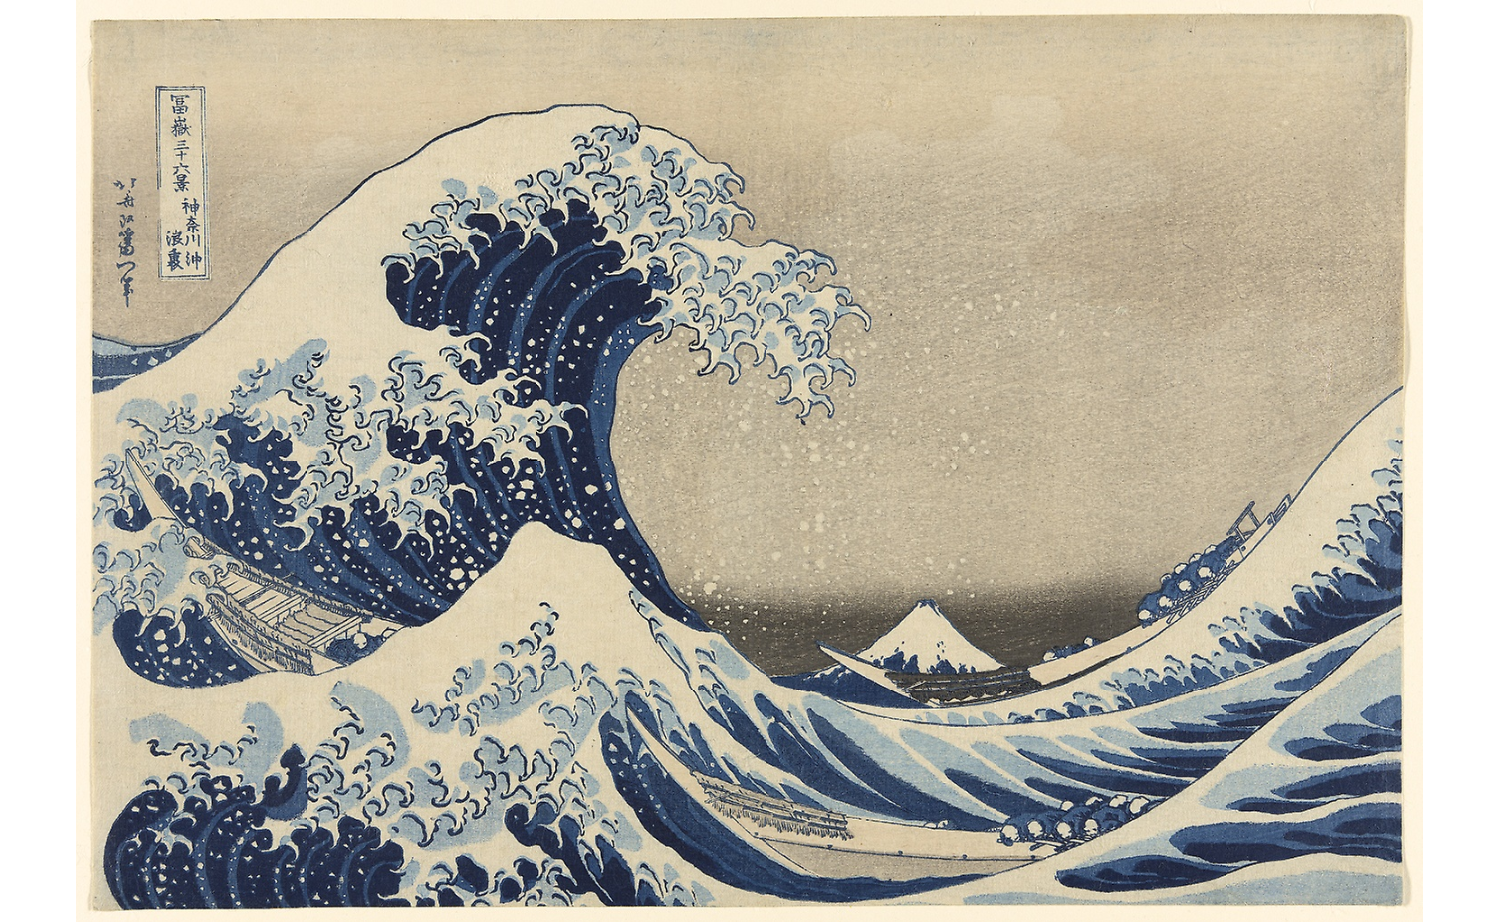
\includegraphics[width=.95\textwidth]{pix/greatwave.png} % 
\end{center}

Kode kompresi citra yang akan kita gunakan terdapat dalam
\inlinecode{img_squeeze.sage}, yang dicantumkan di akhir bab.
Kode ini memecah gambar menjadi tiga matriks untuk data merah, hijau, dan
biru. Kita ingin melihat seberapa parah mutu citra menurun untuk berbagai
nilai batas.
Kode di bawah menetapkan batas dengan hanya mempertahankan suku-suku yang
memuat $10$\% nilai singular terbesar.
Untuk citra ini, sebanyak $92$ nilai singular dipertahankan.
Kode memberi gambaran tentang besarnya nilai-nilai tersebut dengan mencetak
nilai untuk matriks merah (tetapi sebagian besarnya telah kita hilangkan).
\begin{lstlisting}
sage: load("img_squeeze.sage")                                 
sage: img_squeeze("pix/greatwave.png", "pix/greatwave_squeezed.png", 0.10)
citra memiliki 922 baris dan 1497 kolom
sigma_RD 0 =192773.40
sigma_RD 1 =26258.04
sigma_RD 2 =20055.53
sigma_RD 3 =16881.59
sigma_RD 4 =13394.80
sigma_RD 5 =12875.31
sigma_RD 6 =11064.42
sigma_RD 7 =10250.95
    :
sigma_RD 92 =2240.98
\end{lstlisting}
(Sebagai perbandingan, delapan nilai singular terkecil adalah
  $11.22$,
  $10.80$,
  $9.00$,
  $8.26$,
  $8.08$,
  $7.29$,
  $6.55$, dan
  $5.88$.)
Berikut hasil kompresinya.
\begin{center}
  \includegraphics[width=.95\textwidth]{pix/greatwave_squeezed.png}
\end{center}
Gambar ini memperlihatkan hilangnya mutu.
Warnanya tidak sebaik semula, tepinya tidak tajam, dan muncul artefak,
termasuk garis-garis vertikal yang memanjang dari tulisan di kiri atas.
Singkatnya, Fuji menjadi kabur.
Meskipun demikian, citranya tetap sepenuhnya dapat dikenali\Dash hasil yang
tidak buruk setelah menghilangkan $90$~persen suku dalam jumlah tersebut.

Setiap suku tambahan dalam jumlah tersebut menambah kebutuhan penyimpanan
dan transmisi sekitar $2n$ bilangan titik mengambang untuk matriks persegi
berukuran~$\nbyn{n}$.
% The starting image requires $n^2$ floats so we save space is 
% choose a cutoff value less than $0.50$.
Bagi citra $1497\times922$ di atas, batas $0.10$ mempertahankan $92$ suku
dan memerlukan sekitar
$92(1497+922+1)/(1497\cdot922)\approx16\%$ dari jumlah bilangan titik
mengambang pada matriks lengkap, walaupun mutunya mungkin tidak dapat
diterima.
Dengan demikian, memilih parameter batas merupakan keputusan rekayasa:
pada rentang antara ketepatan dan konsumsi sumber daya, Anda memilih nilai
yang sesuai dengan penerapan Anda.
 
Menetapkan parameter batas ke~$0.20$ dapat menghasilkan citra keluaran yang
sulit dibedakan dari citra asli.
Di bawah ini terdapat gambar Suzy dari sampul panduan ini.
Di sebelah kiri adalah citra asli, sedangkan di sebelah kanan adalah citra
yang dikompresi dengan nilai parameter~$0.20$ (keduanya ditampilkan pada
$40$\% ukuran penuhnya).
\begin{center}
  \vcenteredhbox{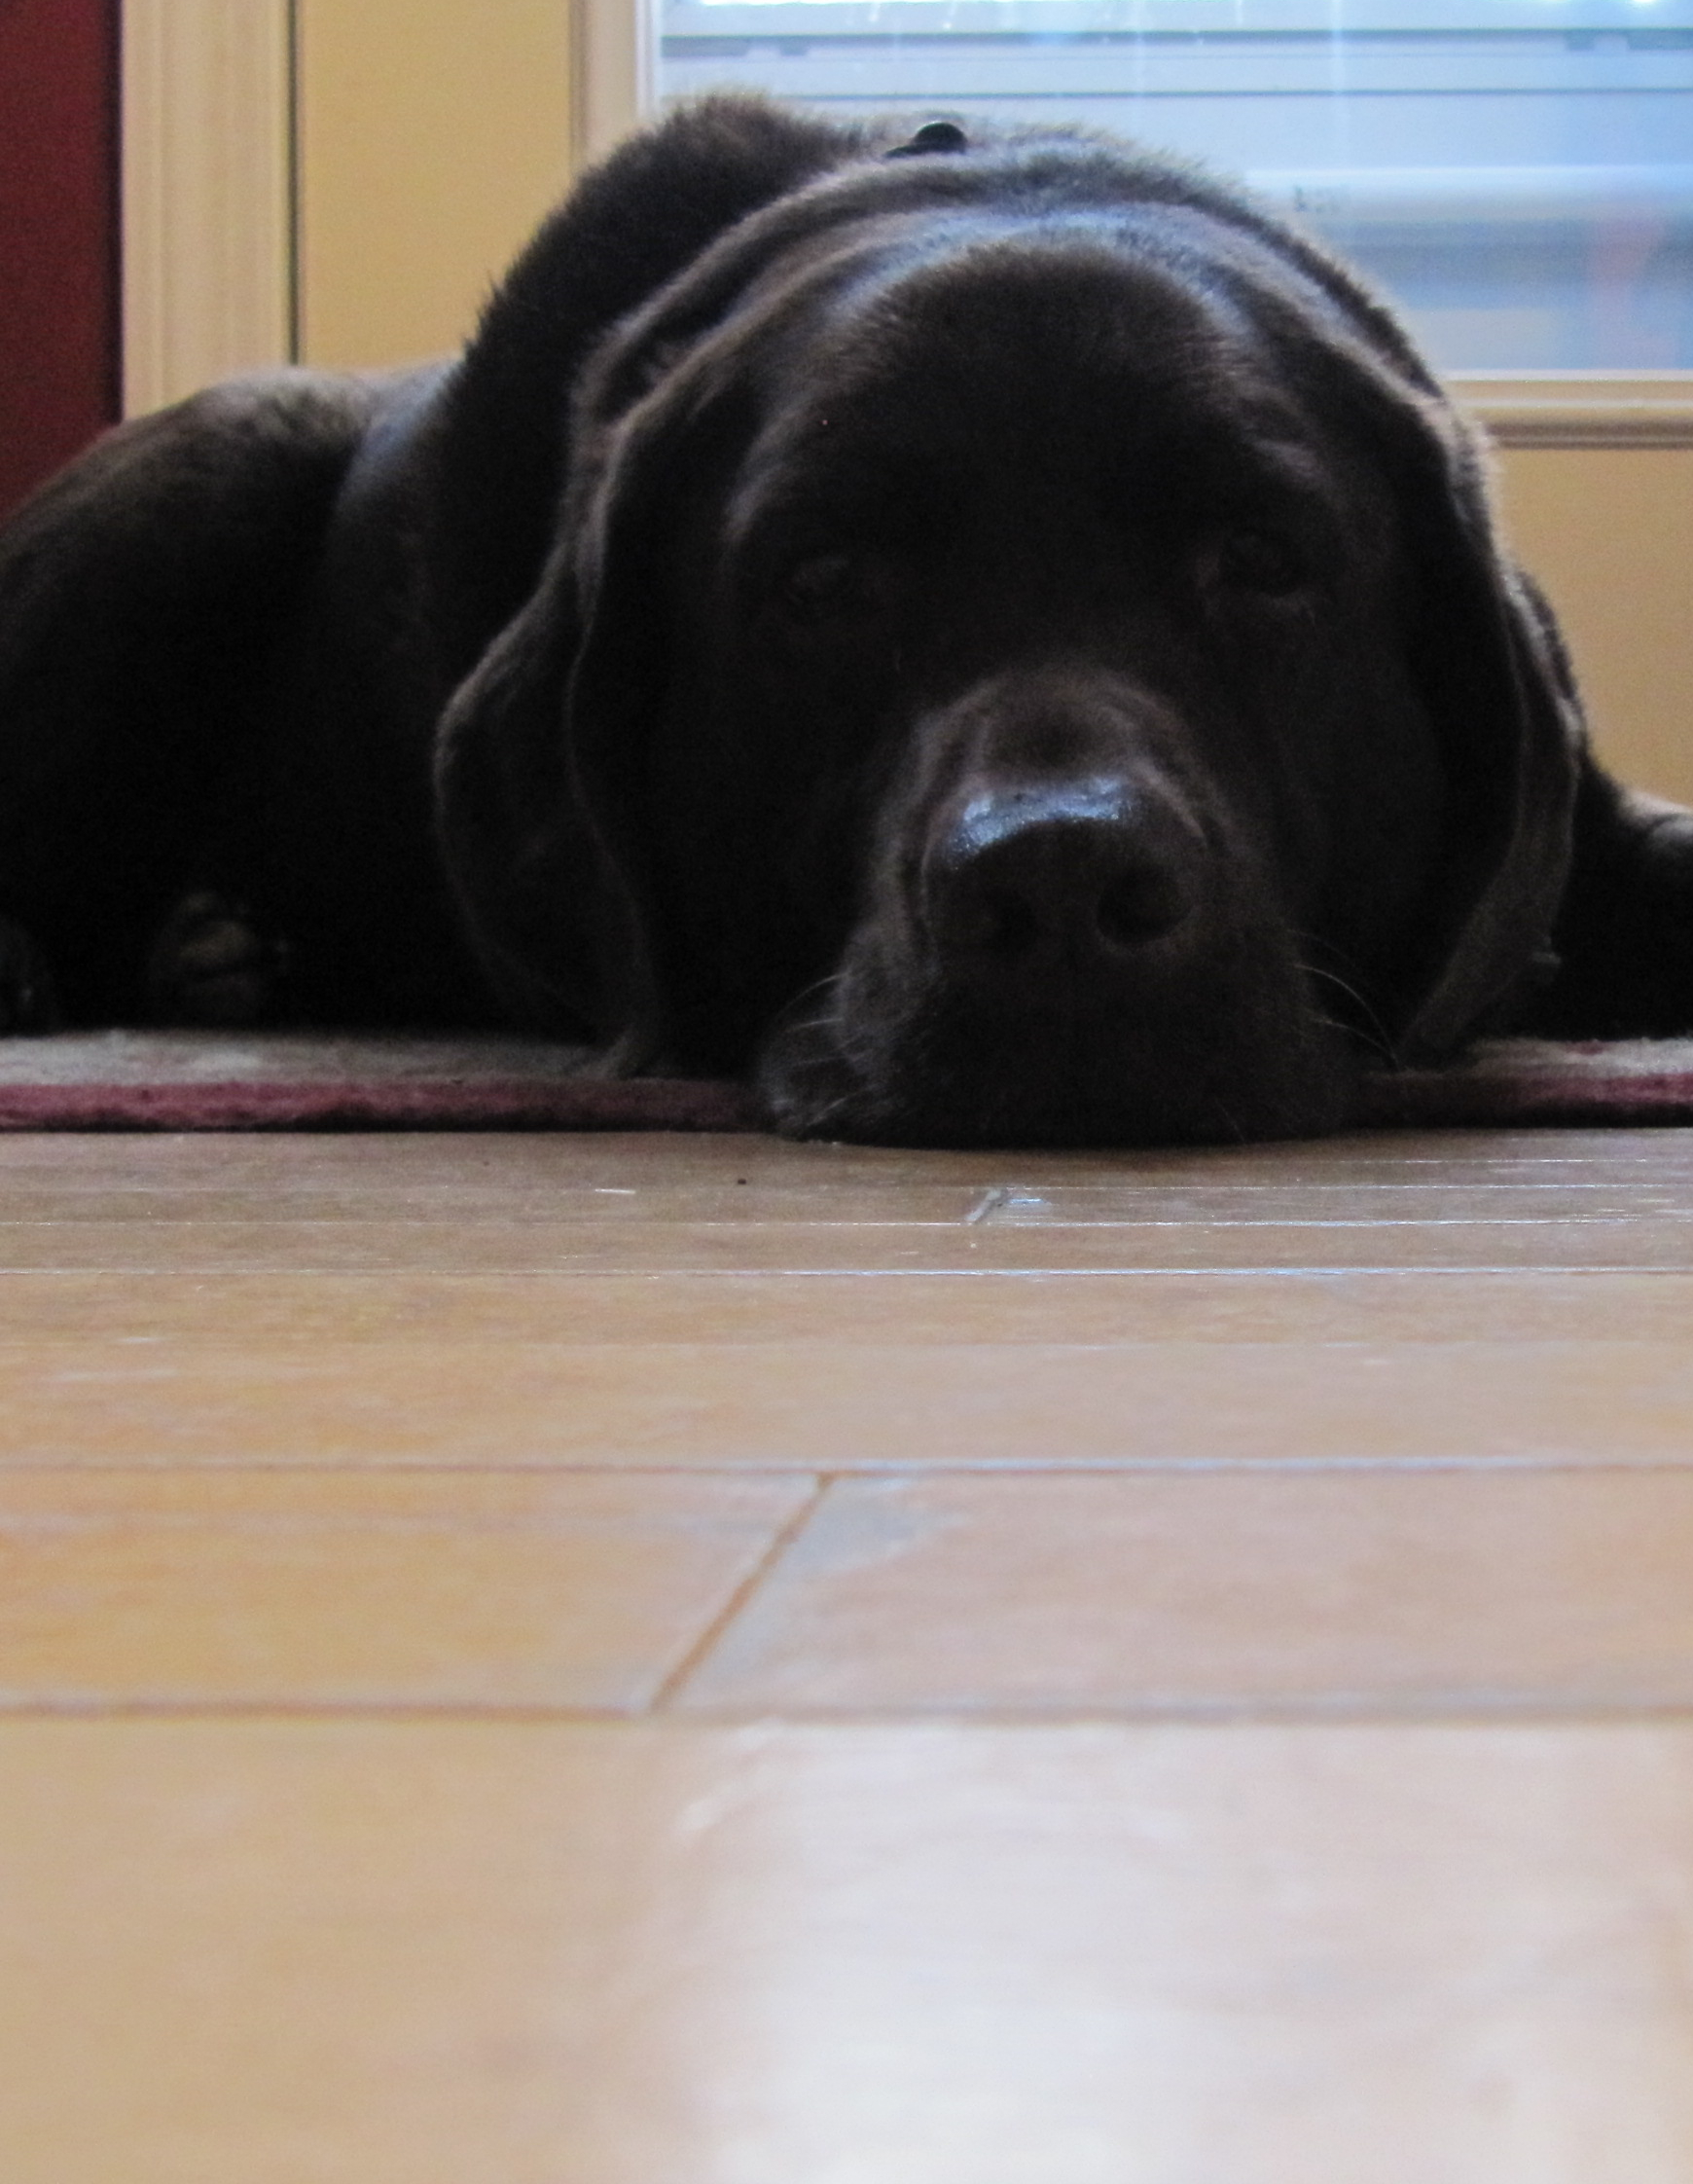
\includegraphics[width=.4\textwidth]{pix/suzy_cover.png}}
  \quad
  \vcenteredhbox{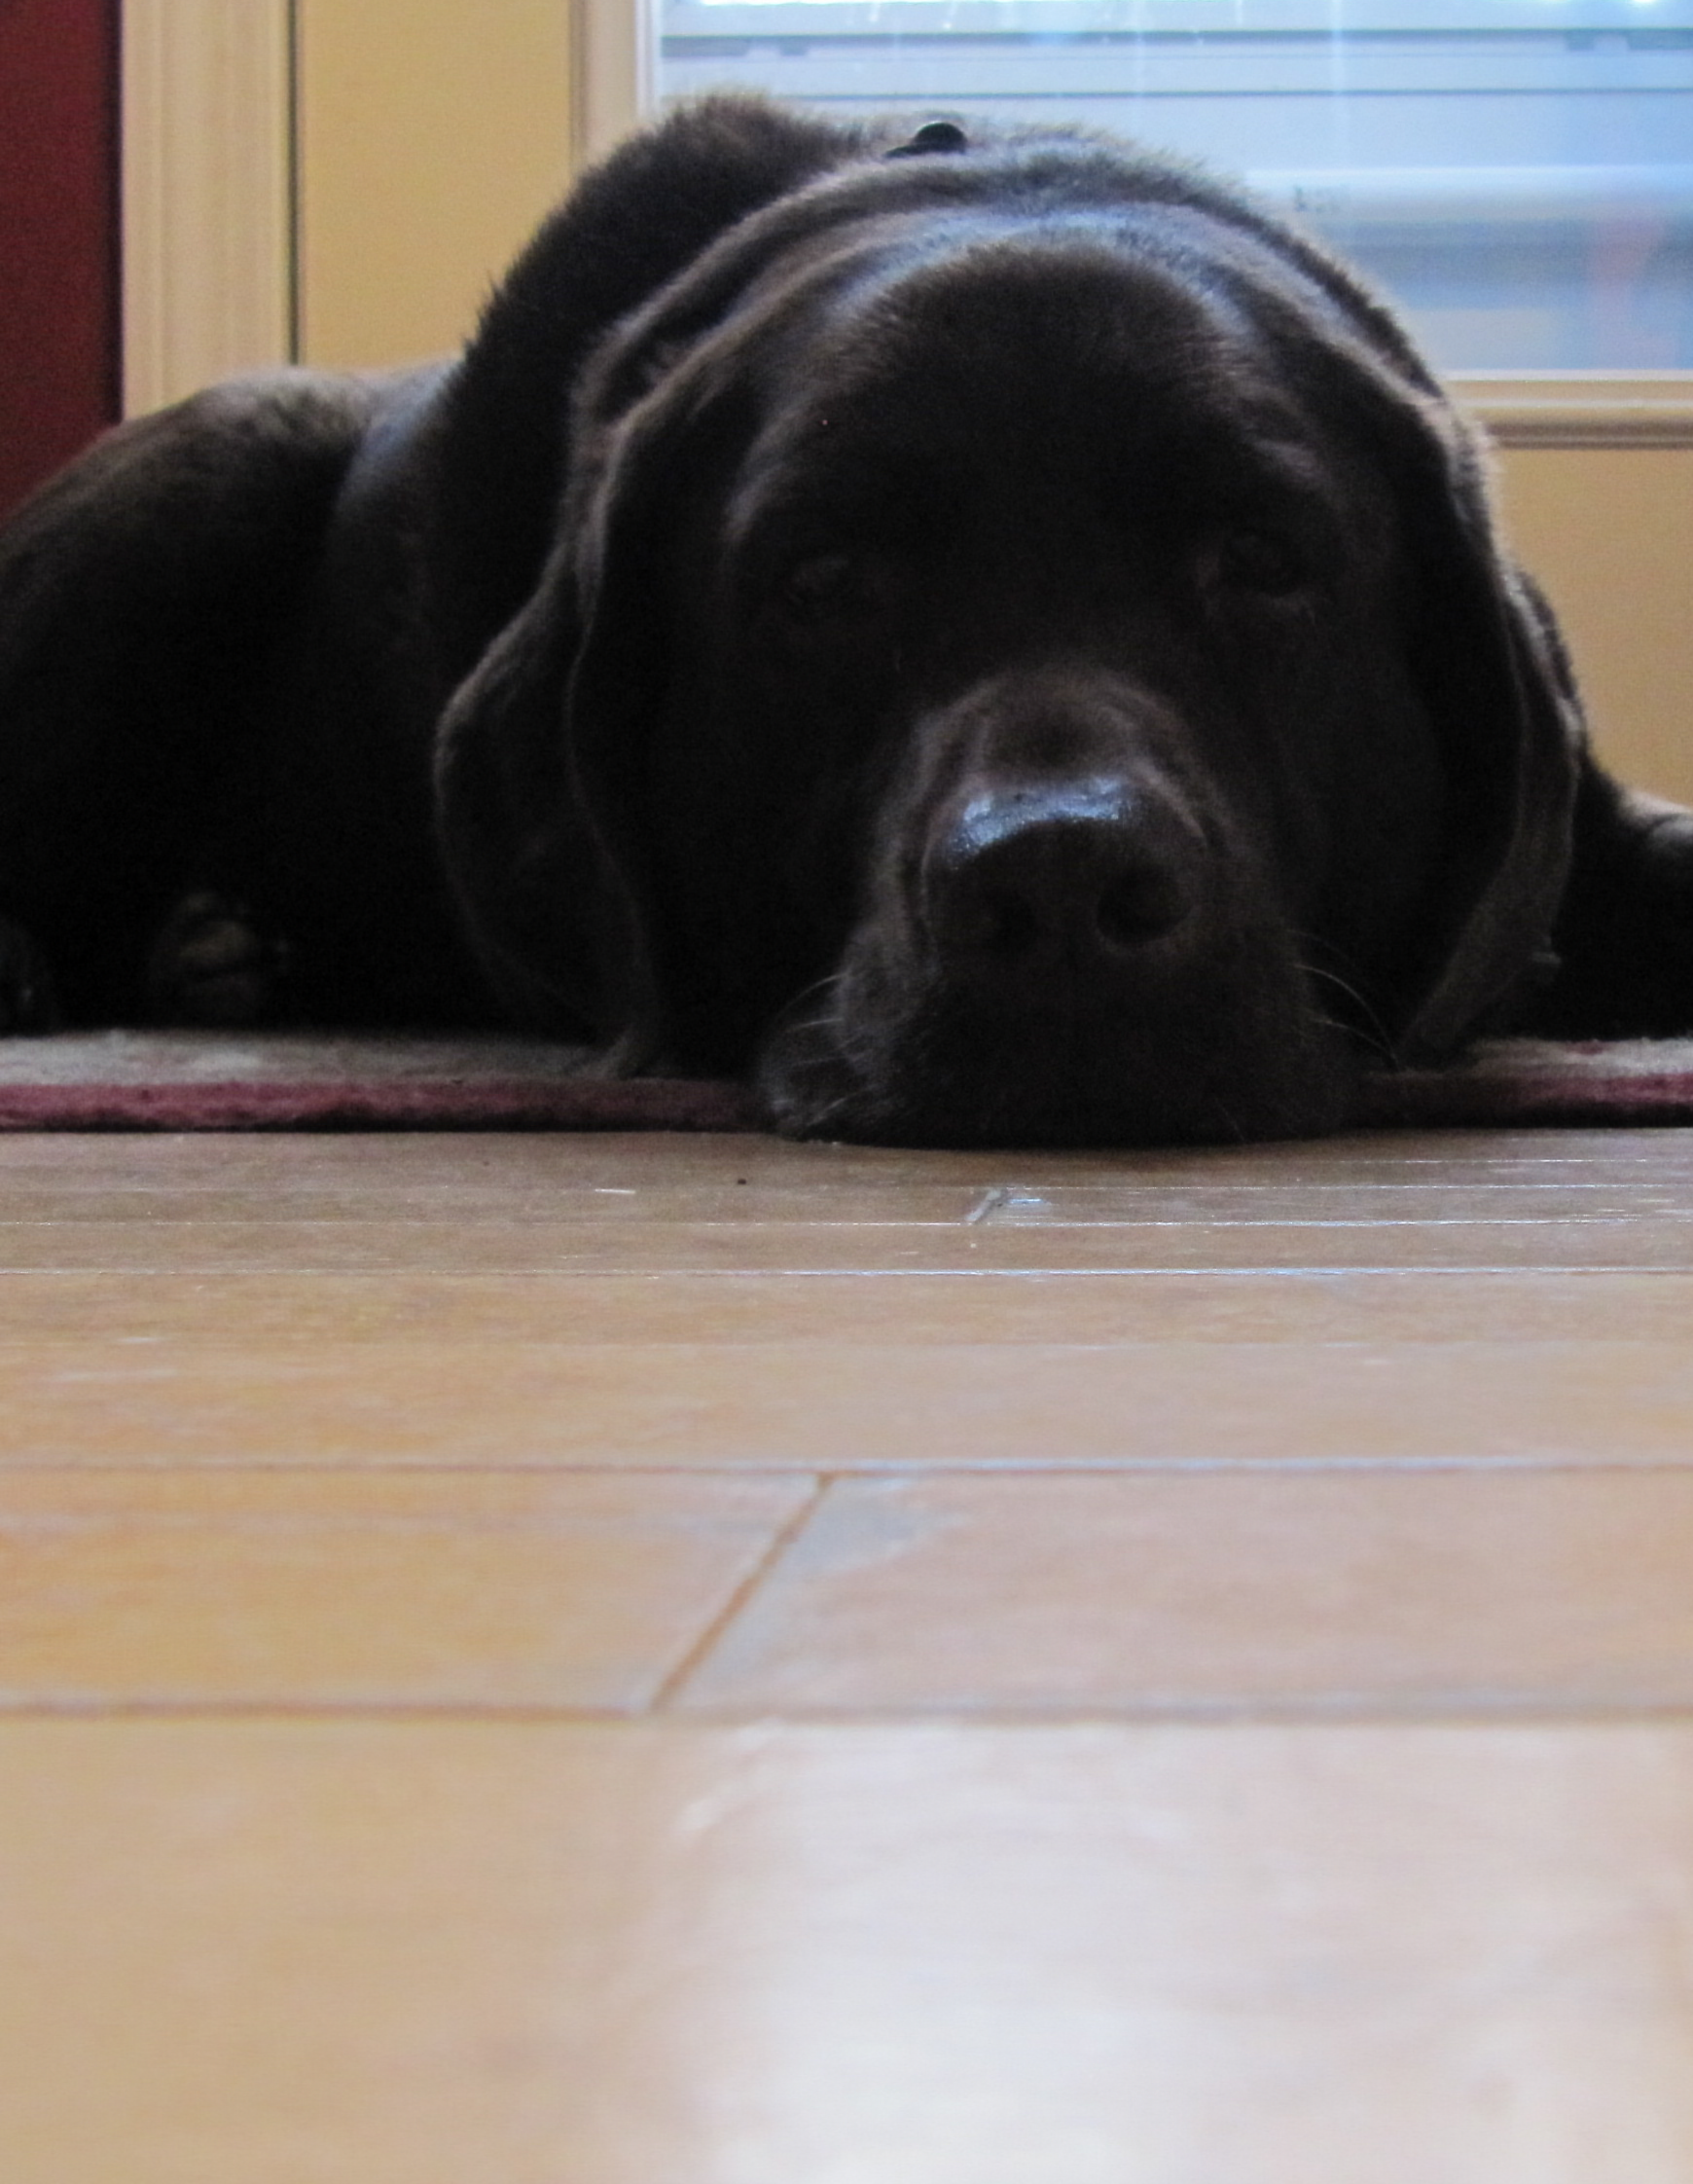
\includegraphics[width=.4\textwidth]{pix/suzy_cover_squeezed.png}}
\end{center}
(Nilai singular terbesar adalah
$291533.51$.
% $39038.59$,
% $30526.84$,
% $19983.01$,
% $13946.40$,
% $11523.07$,
% $9354.02$, and
% $8067.98$.
Batas dua puluh persen adalah $129.23$.
Nilai terkecil dari $1739$ nilai singular adalah $3.36$.)
Berkas PNG di sebelah kiri berukuran $4$~megabita, sedangkan yang di sebelah
kanan berukuran~$3.4$~megabita; perbandingan ukuran berkas ini juga dipengaruhi
oleh kompresi internal format PNG dan bukan ukuran penyimpanan faktor SVD
semata.


\section{Kode sumber plot\_action.sage}

Rutin \inlinecode{plot_circle_action} menerima keempat entri matriks
$\nbyn{2}$ dan menghasilkan sebuah grafik keluaran.
Untuk membuat pasangan gambar masukan dan keluaran seperti di atas, rutin
dipanggil sekali dengan matriks identitas dan sekali dengan matriks
transformasi. Parameter lainnya adalah banyaknya warna dan sebuah penanda
yang menentukan apakah lingkaran penuh atau hanya setengah lingkaran bagian
atas yang diplot.

Rutin pengendali menghitung daftar warna dan memanggil rutin pembantu
\inlinecode{color_circle_list} yang diberikan di bawah; rutin pembantu ini
menghasilkan sebuah daftar grafik.
Terakhir, rutin pengendali memplot grafik-grafik tersebut (operator
\inlinecode{+=} menambahkan gambar di sebelah kanan ke grafik yang telah
tersimpan di sebelah kiri).
\lstinputlisting[firstline=39,lastline=50]{plot_action.sage}

Rutin pembantu melakukan pekerjaan utamanya.
Ada dua variabel global.
Variabel \inlinecode{CIRCLE_THICKNESS} menetapkan ketebalan pena yang
menggambar kurva, dalam poin (satuan percetakan sebesar $1/72$~inci).
Variabel \inlinecode{DOT_SIZE} menetapkan jari-jari lingkaran kecil yang
kosong, dalam satuan koordinat grafik.
Rutin ini menghasilkan kurva berparameter $(x(t),y(t))$ dan menggunakan
fungsi \inlinecode{parametric_plot} milik \Sage{} untuk menghasilkan
grafiknya.
\lstinputlisting[firstline=5,lastline=36]{plot_action.sage}
Jika rutin ini memplot setengah lingkaran bagian atas, rutin tersebut
menambahkan lingkaran kecil kosong di ujung untuk menunjukkan bahwa bayangan
$(-1,0)$ bukan bagian dari grafik.




\section{Kode sumber img\_squeeze.sage}
Kita menggunakan Python Imaging Library untuk membaca dan menulis citra.
\lstinputlisting[firstline=6,lastline=6]{img_squeeze.sage}
Fungsi \inlinecode{img_squeeze} menerima tiga argumen:~nama kedua berkas dan
bilangan riil batas antara $0$ dan~$1$ yang menentukan proporsi nilai
singular yang dipertahankan dalam jumlah.
\lstinputlisting[firstline=8,lastline=12]{img_squeeze.sage}

Mula-mula, fungsi ini mengubah data masukan ke format yang menyatakan setiap
piksel sebagai tripel bilangan bulat
$(\text{merah},\text{hijau},\text{biru})$, dengan nilai antara $0$ dan~$255$.
Fungsi tersebut menggunakan bilangan-bilangan ini untuk membangun tiga larik
Python \inlinecode{rd}, \inlinecode{gr}, dan \inlinecode{bl}, yang kemudian
menginisialisasi tiga matriks \Sage{}, yaitu \inlinecode{RD},
\inlinecode{GR}, dan~\inlinecode{BL}.
\lstinputlisting[firstline=13,lastline=29]{img_squeeze.sage}

Langkah berikutnya mencari Dekomposisi Nilai Singular ketiga matriks itu.
Sebagai informasi tambahan, kita melihat delapan nilai singular terbesar
dalam matriks merah, nilai singular pada batas pemotongan, dan delapan nilai
singular terkecil.
\lstinputlisting[firstline=30,lastline=41]{img_squeeze.sage}

Terakhir, untuk setiap matriks kita menghitung jumlah
$\sigma_1\cdot\vec{u}_1\trans{\vec{v}}_1+\sigma_2\cdot\vec{u}_2\trans{\vec{v}}_2
   +\cdots\,$,
hingga indeks sebelum batas pemotongan.
\lstinputlisting[firstline=42,lastline=61]{img_squeeze.sage}

Sebagai penutup, kita memasukkan data ke format PNG dan menyimpannya ke
media penyimpanan.
\lstinputlisting[firstline=62,lastline=70]{img_squeeze.sage}
(Bagian rutin ini memerlukan waktu cukup lama, beberapa detik, antara lain
karena kode tersebut dirancang agar mudah dibaca dan bukan agar berjalan
secepat mungkin.)

\endinput
